\documentclass[fyp]{socreport}
\usepackage{fullpage}
\usepackage{parskip}
\usepackage{amsmath}
\usepackage{MnSymbol}
\usepackage{graphicx}
\usepackage{wrapfig}

\usepackage[usenames,dvipsnames,svgnames,table]{xcolor}
\usepackage[english]{babel}
\usepackage[
backend=biber,
style=alphabetic,
sorting=ynt
]{biblatex}
\addbibresource{socreport.bib}

\usepackage{titlesec}
%\titleformat{\subsection}[runin]
%  {\normalfont\large\bfseries}{\thesubsection}{1em}{}
\titleformat{\subsubsection}[runin]
  {\normalfont\normalsize\bfseries}{\thesubsubsection}{1em}{}

\begin{document}
\pagenumbering{roman}

\title{Hands-Free Programming - Talk to Code}
\author{Soon Chun Mun}
\projyear{2015/16}
\projnumber{H0201120}
\advisor{Prof. Ooi Wei Tsang}

\deliverables{
  \item Report: 1 Volume}
\maketitle

\newcommand{\vp}{$\vphantom{equals to}$}
\newcommand{\tagw}[3]{$\underbrace{\hbox{\vp #1}}_{\hbox{\color{#3} \vp \textbf{#2}}}$}
\newcommand{\tago}[1]{\tagw{#1}{O}{Grey}}
\newcommand{\tagfor}[1]{\tagw{#1}{for}{red}}
\newcommand{\tagfi}[1]{\tagw{#1}{iters}{red}}

\newcommand{\tagfn}[1]{\tagw{#1}{fn-name}{Blue}}

\newcommand{\tagcond}[1]{\tagw{#1}{cond}{blue}}
\newcommand{\tagif}[1]{\tagw{#1}{if}{blue}}
\newcommand{\tagvn}[1]{$\underbrace{\hbox{\vp #1}}_{\hbox{\vp \textbf{{\color{ForestGreen} var}-name}}}$}
\newcommand{\tagvv}[1]{$\underbrace{\hbox{\vp #1}}_{\hbox{\vp \textbf{{\color{ForestGreen} var}-val}}}$}
\newcommand{\tagvm}[1]{$\underbrace{\hbox{\vp #1}}_{\hbox{\vp \textbf{{\color{ForestGreen} var}-mod}}}$}
\newcommand{\tagva}[1]{$\underbrace{\hbox{\vp #1}}_{\hbox{\vp \textbf{{\color{ForestGreen} var}-ass}}}$}

\begin{abstract}

In this report, we explore a method to identify semantic roles within
transcribed text as part of a pipeline to turn spoken speech into
code. The problem involves extracting the words that form the components
of code and command by correctly labelling them in their various semantic
context.

\begin{descriptors}
    \item C5 Computer System Implementation
\end{descriptors}
\begin{keywords}
	Semantic Role Labelling, Natural Language Processing, Neural Network
\end{keywords}
\begin{implement}
	Python 3.5.1 Theano 0.7
\end{implement}
\end{abstract}

\begin{acknowledgement}
   I would like to thank my friends, families and advisors.
   Without them, I would not have be able to complete this project.
\end{acknowledgement}



\listoffigures
\listoftables
\tableofcontents

\chapter{Introduction}

\section{Background}
This project embarks on constructing a possible framework which human
programmers are able to use speech to directly write code instead of typing
them. Conversion of human speech to code requires an understanding of code
structure occur in spoken code.

The code structures that we explored involved variable declaration, loops,
if-else conditions and function declarations.

Although spoken code contains nuances of natural humans language, we discovered
that the structures are syntactically very close to actual written code. In
fact even when humans express code that is not syntactically correct, it seems
that the number of ways they are spoken is very consistent and similar.  For
example, in the construction of a \texttt{for} loop. Many may choose to
express in the following ways:

\begin{verbatim}
  1. for i equals to 0 i less than 10 i plus plus
  2. for loop that runs 10 times
  3. create a for loop inside that runs 10 times
\end{verbatim}

We see that although the first sentence is an accurate reflection of how code
may be written as it is spoken, the second version is equally likely to occur.
The second version is a lot more natural even though it fails to specify the
loop variable or invariants because that has been abstracted away when the main
purpose of the code is to run a loop a number of times.

The last example is a sentence which we extracted from the transcribed corpus
that we used with our experiments. We see that the sentence contains
additional semantic context such as an explicit creation of the loop and that
the code within the loop should run 10 times.

All 3 examples clearly expresses the idea of creating a for loop that runs a
set number of times and our project intends to finally output C code that is
very similar to the first sentence. However, there are enough differences
between them that this cannot be directly approached without considering
the robustness of the method of translation in the presence of missing
information or word paraphrasing in non-programming keywords.

This motivates us to model the problem in terms of \textbf{Semantic Role
Labelling} where semantically relevant keywords of the given sentence are
identified before further processing can infer missing information.

\section{The Problem}

The problem we tackle here involves the part of the pipeline where accurately
transcribed text is labelled with semantic tags such as \texttt{variable-name},
or \texttt{if}. The model which is adopted is a sequence prediction given
the sentence. The predicted sequence represents the sequence of semantic tags.

\begin{enumerate}
\itemsep0em
  \item \tagfor{for} \tagvn{i} \tagva{equals to} \tagvv{0} \tagvn{i} \tagcond{less than}
    \tagvv{10} \tagvn{i} \tagvm{plus plus}
  \item \tagfor{for} loop that runs \tagfi{10} times
  \item create a \tagfor{for} loop inside that runs \tagfi{10} times
\end{enumerate}

To change the tagged sequence so that it is the same length as the input
sentence, we have to split tags that have contiguous words into separate tags
as well as have placeholder for non-tagged word. We are able to have tagged
sequence that is of the same length, like the below for the last line.

\hspace{20pt}
\tagfor{for} \tago{loop} \tago{that} \tago{runs} \tagfi{10} \tago{times}

The approach we are taking fits into a sequence-to-sequence modelling task
naturally. We will use a neural network approach to solve this task.
Specifically, we use a Recursive neural network that reads the sentences in one
word at a time and generates the tags after every word. Now the sentence
length and the tag sequence length are the same by artificially adding in the
dummy tag.


\section{Our Solution}
Recurrent neural networks has produced many impressive results on speech and
natural language processing as well computer vision task. These tasks are
characterized by an extremely large dimension space of the model. In our
specific task of sequence-to-sequence prediction, if we have $w$ words, and
$t$ different tag, then a sentence of length $n$ will have an input space
of $w^n$ and an output space of $t^n$. A large percentage of the input sentences
will be invalid because they do not make any sense in English as well as
invalid tag sequences in the output. However, this does not make this
task any less daunting given that there can be a complex combinations of words
that code can be expressed in speech.

Our approach is basically a supervised learning machine learning task. After
creating a corpus of correctly labelled sentences, we train the recurrent
neural network by feeding in each word in a sentence sequentially into the LSTM
and reading a tag at each time step. The process can be roughly abstracted as
shown in the figure:

\begin{figure}[h]
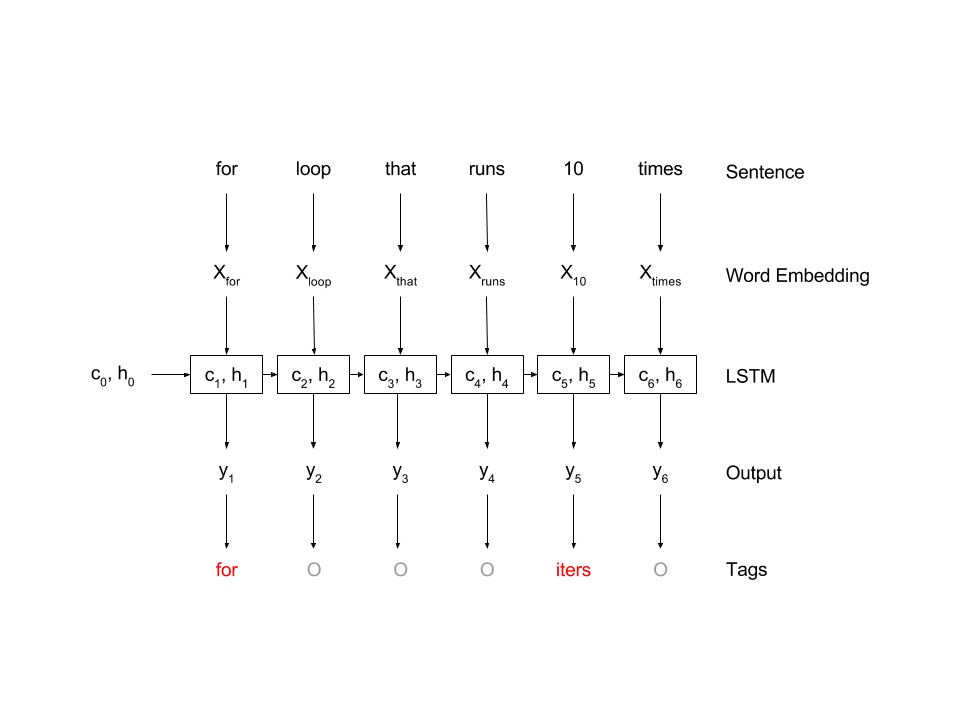
\includegraphics[width=\textwidth]{Workflow.png}
\caption{Workflow for tagging a single sentence.
$c_0$ and $h_0$ represents the initial internal states of the LSTM.}
\centering
\end{figure}

The internal states of the LSTM persists between the input each word
embedding vector in the sentence. Note that here, we apply each word
to the LSTM sequentially rather than in one long sentence vector as
how most convolutional sequence-to-sequence models generally work. The
internal states only persist between inputs within a sentence. They are
reset when we need to parse the next sentence.

\subsection{Corpus}
We have gathered a small corpus of 500 labelled sentences that is used for
supervised training. Students, who are programmers, are given 4 different tasks
in which they must express their code by speaking directly to an experimenter.
The experimenter will listen to what the student said, and proceed to type on
the computer what is interpreted from his speech. The speech is generally a mixture
of movement commands as well as code definitions, such as variable declaration.
Throughout the entire experiment, the student is not able to directly type or
gesture to the experimenter his intent other than through his or her own voice.

After each person has completed their task, their speech is then transcribed
and tagged manually. The sentences boundaries are inserted whenever the student's
speech reached an extended pause. This creates the realistic situation of
a real-time parsing of the spoken code. However, it also created many situations
where the spoken utterance did not contain any semantic elements like filler
words.

Since the programming task is known beforehand, we can easily infer the intent
of the spoken programme just by reading from the transcribed sentence. For example,
we differentiated between the word \texttt{number} in these 3 different context.

\begin{enumerate}
\itemsep0em
  \item \tago{go} \tago{to} \tago{line} \tago{number} \tago{7}
  \item \tagw{if}{if}{Blue} \tago{the} \tagvn{number} \tagfn{mod}
    \tagvv{2} \tago{is} \tago{even}
  \item \tagfn{printf} \tago{the} \tago{number} \tago{is} \tago{even}
\end{enumerate}

In the first sentence and in the last sentence, \texttt{number} is tagged
with the dummy tag. However, in the second case, the correct tag is
\texttt{variable-name}.

If the sentence are taken out of context, even humans will have a difficult
time tagging this.  We can easily compound the problem if all the 3 sentences
are combined into a single sentence. A student might indicate his wish to move
to the 7th line, followed by a \texttt{if} conditional and a \texttt{printf}.

It will be difficult for sequence-to-sequence predictors to figure out what the
correct tags are without considering the surrounding word context and sentence
structure. Especially so when the same word is tagged differently. The system
must be robust to arbitrary combinations of the statements. However, the size
of the labelled corpus severely restricts the number of examples that the model
has been trained on and causes over-fitting to happen when the examples are
sparse.

\subsubsection{Vocabulary Sparsity} For example, given the complexity of the
model parameters and small number of variable names seen, the model might
over-fit by remembering that some words are very likely to be variable names
compared to others. Words that are not seen before have a high chance of being
tagged with the dummy tag even though they may occur with high probability with
same tags like \texttt{variable-names}. Hence the problem faced by a small
corpus consists of 2 parts, one, the lack of sufficient examples in the
structure of spoken code, and two, the limited vocabulary of the corpus.  We
shall discuss this problem in further depth during the presentation of the
results.

% TODO : Talk about how the generated corpus is useless

\subsubsection{Generated Corpus}
In the initial parts of the project, we set up to mitigate some of the issues
of corpus sparsity by generating an artificial corpus that contains an arbitrary
combination of certain code structures that we predict will appear in spoken code.

For example, we can easily create a corpus with a sentence prototype like so:

\hspace{20pt}
\tagif{if} \tagvn{i/j/k/...} \tagcond{less than/greater than} \tagvn{i/j/k/...}

This method helped to alleviate some of the sparsity problem that occurred in
the tagged transcribed speech. The corpus is now expanded with more possible
patterns of spoken code. However, this does not alleviate the problem of limited
vocabulary very much at all. Moreover, we see that the sentences in human spoken
code is punctuated with many dummy tags, but the generated corpus lacks such
features.

With just 15 sentence prototypes, the combinatoric explosion in the possible
combinations exceed over 30k sentences - Overwhelming the manually annotated
sentence count 65 to 1. The generated sentences are attached to the training
set together with the manually annotated sentences.

% TODO : Talk how about a modified version of dropout is used vs normal dropout
% TODO : Dropout by replacing with rare tag randomly
% TODO : Check ability to generalize
\subsubsection{Dropout} The concept of dropout is employed at the word
embedding level and the output layer. After the words are transformed into
their word vector embeddings, half of the vector is randomly zero-ed based on a
50\% probability. This closely follows the dropout scheme that was formulated
by \cite{2014Zaremba} so that the training of the RNN is not affected by
dropouts in between the gates.

\subsection{Word Embeddings}
First the words of the sentence are converted to word vectors via a word
embedding. The word embedding used in all our experiments is a float vector of
length 50. In our solution, the embedding vectors are randomly generated
initially before being updated using the back-propagated gradients during the
update step. A special \texttt{<unk>} symbol is given to words that we did not
encounter within the training corpus. We adopted word embeddings in our
training in the hope that similar words that have the same tags will be "close
together" in the word embedding space.

Here we also experimented with using pre-trained word embeddings from Wikipedia
that is trained using Glove \cite{pennington2014glove}.

After converting the words in the sentence into word vectors, we then feed the
word vectors one at each time step into the LSTM.

\begin{figure}[h]
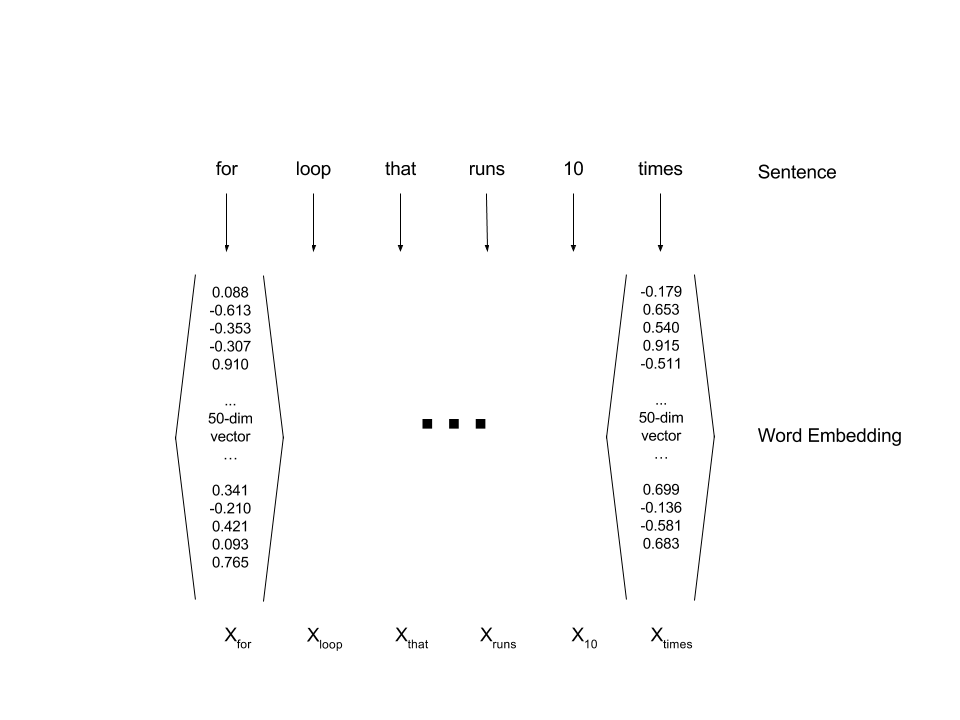
\includegraphics[width=\textwidth]{embedding.png}
\caption{The word vectors are randomly generated for each word initially}
\centering
\end{figure}

% TODO : Lemmatization
There are approximately 500 words present in the words that were annotated within
our experiments. The dimensionality is small enough that lemmatization did
not significantly alter the performance of our solution. On the other hand, the
pre-trained Glove embeddings, comes with a much larger vocabulary size of
around 30k words.

Using pre-trained word vectors helped to improve the convergence of the model
training. However, the key here is that we need to continuously update the
word embedding vectors. As observed in the final results, a fixed word embedding
that is pre-trained on an out-of-domain corpus produces worse convergence rates
for model training, performing worse than random initialization.

This negates some of the benefits of using a larger pre-trained corpus with the
hopes that rare words can be infered more accurately against the seen vocabulary
when the words are close in the word embedding space. Since we update and
modify the word embeddings of the words in our training set, the simiarity
constraint is no longer preserved.


\subsection{LSTM}
Long-short term memory (LSTM) refers to a specific architecture of Recursive
neural networks that is arranged as follows:


$\sigma$ is the sigmoid function $f(x) = \frac{1}{(1 + e^x)}$, $\odot$ is the
matrix element-wise multiplication. We can then represent all the updates
made on the hidden state $c_t$ at time step $t$ given the input $x_t$.
{
\begin{wrapfigure}{l}{0.8\textwidth}
    \centering
    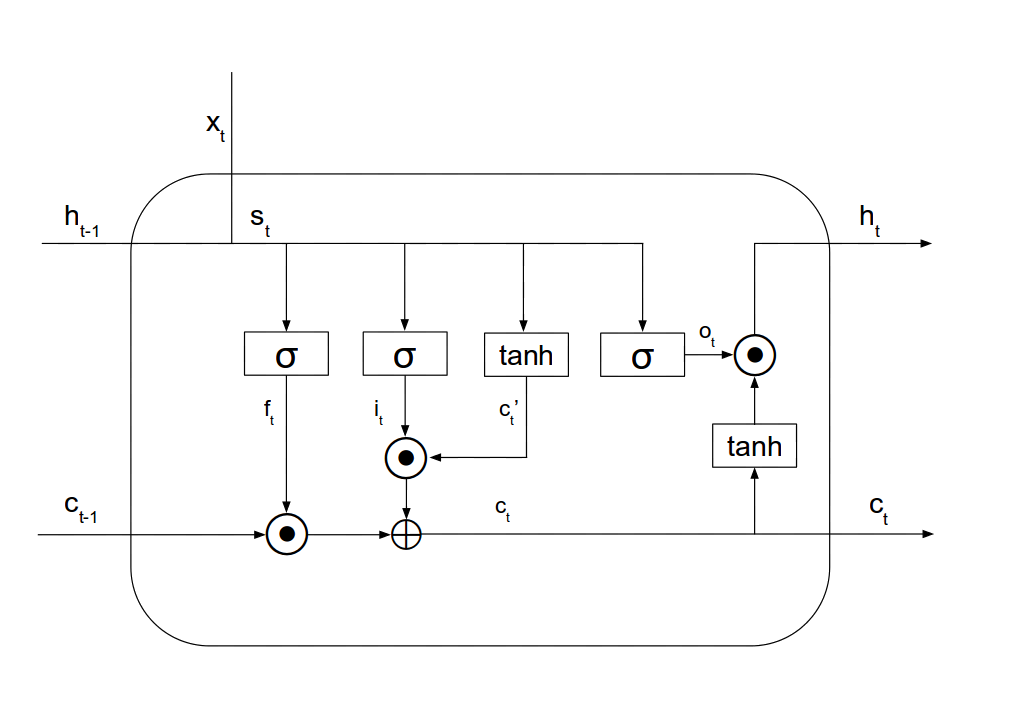
\includegraphics[width=0.8\textwidth]{LSTM.png}
    \caption{Diagram of internal operations in an LSTM cell at time step $t$}
\end{wrapfigure}

% TODO : LSTM Figure
\begin{align*}
  \\
  s_t &= \lbrack h_{t-1}, x_{t} \rbrack \\
  f_t &= \sigma \left( W_f s_t + b_f \right) \\
  i_t &= \sigma \left( W_i s_t + b_i \right) \\
  c_t' &= tanh \left( W_c s_t + b_c \right) \\
  o_t &= \sigma \left( W_o s_t + b_o \right) \\
  c_t &= c_{t-1} \odot f_t + i_t \odot c_t' \\
  h_t &= o_t \odot tanh \left( c_t \right) \\
  y_t &= softmax \left( h_t W_s + b_s \right) \\
\end{align*}
}

At each word, the internal hidden states $c_t$ is updated as it advances from
one word to the next by removing irrelevant information and incorporating
new information.

We added another layer of linear operation on the output state $h_t$ to get
$y_t$ before we are able to evaluate the softmax. This effectively frees the
LSTM to have the size of the hidden vector $c_t$ to be the same as the output
$y_t$. Adding another sigmoid operator on $y_t$ seems to have yielded extremely
bad training results that does not converge fast enough. This could be a case
of bad initialization of the output layer, but we did not have sufficient time
to fully test our hypothesis.

The appeal of using a Recursive neural network like the LSTM over more
conventional methods like convolutional networks or fully connected neural
networks is that the input sequence can be made arbitrarily long, while still
retaining the capability of learning long range dependencies.


\chapter{Related Work}
\section{SENNA}
The de facto Semantic Role labelling framework that provided a similar
neural network approach to the \cite{DBLP2011Collobert}

\section{Bi-directional LSTM-CNNs-CRF}


\section{Statistical Machine Translation}
There is an equally appealing framework for


\label{ch:related}


\chapter{Problem and Algorithm}
\section{Formal Description of Problem}
After defining the problem in terms of a sequence prediction, we now state the
loss function that is used as a measure of how likely the correct sequence of
tags are predicted given the input.

\subsubsection{Loss Function} We measure the how well the model does by the
negative log likelihood of the labelled tagged sequence when given the
conditional probability of all tags for each word. This is the same loss
function that will be optimized during the learning of the model parameters
$\theta$. The parameters refer to the weight and bias matrices that are used
the LSTM. Given a word $w \in W$ from the list of words in our vocabulary, we
obtain a probability of $P(T=t | w, \theta)$ for every given tag that exists in
our system.
\begin{equation}
  \ell(\theta) = -\sum_{w \in W} \sum_{t \in T} log(P(t | w, \theta)) I(t = \hat{t})
\end{equation}
where $\hat{t}$ is the correct tag for $w$ and $I$ is the 0-1 loss function

\subsection{Word Level Likelihood}

The loss function defined here is extremely similar to the one presented by
Collobert \cite{DBLP2011Collobert} under the section of Word-Level log
likelihood. This formulation just results in the correct path being having
increased likelihood but does not take into account of sentence level tag
dependencies that is captured in a more sophisticated sentence likelihood
function.

In brief, the sentence likelihood function considers a probability function
which places an explicit cost for certain tag-to-tag transitions. The extension
which was proposed in the paper involved learning the transition probability
and then producing a Sentence level log likelihood loss function. The best
sentence is optimal decoding over all possible paths that the tag sequence that
take using the Viterbi algorithm.

A more recent approach that is taken by the Xuezhe \cite{2016arXiv160301354M}
is to add a Conditional Random Field layer on top of the output of their
Bi-directional LSTM layer. This allows the final output to take into
consideration tag transitions given the hidden states that is
generated from the 2 LSTMs in both directions.


\section{Design of Algorithm}

\subsection{Training}

\subsubsection{Stocastic Gradient Descent} The optimization of the function is
done by employing gradient descent over the parameters in the LSTM (including
the word embedding vector).

Taking the gradients of the contribution of each weight and bias matrix is
easily done in Theano by using the Tensor gradient function. We make of this
functionality as well when defining the version of the loss function with the
L2 regularization term. The only hyperparameter that needed to be determined
here is the learning rate $lr$.
\begin{equation}
  \theta \leftarrow \theta - lr * \frac{Loss}{\delta \theta}
\end{equation}

\subsubsection{AdaDelta} We find that implementing AdaDelta where we take sums
of the historical gradients helped out result to converge much faster than just
using SGD without momentum. The resulting modified gradient descent is the one
that we will be using in the experiments. However, this method introduced another
hyperparameter $\rho$ that needs to be tuned for the convergence to work well.

We discovered that a $\rho$ and $lr$ value of 10 and 1 works best after some
random searching.
\begin{align*}
  h &\leftarrow h + \left( \frac{\partial \ell(\theta)}{\partial \theta} \right)^2 \\
  \theta &\leftarrow \theta - lr * \frac{\partial \ell(\theta)}{\partial \theta}
  * \frac{\rho}{\rho + h}
\end{align*}

There is several literature and advances on different gradient descent
technique such as AdaGrad, RMSProp and Nesterov method.  However, there are
different appropriate initialization parameters for the weight matrices for
each technique.  Exploration of the different gradient descent techniques
are out of scope for this project but we feel the significantly faster rate of
convergence due to AdaDelta deserved a special mention.

\subsubsection{Gradient Clipping} In order to prevent fluctuations of the parameters
values, we employ a method called clipping on the gradient matrices $h$ and
$\frac{\partial \ell(\theta)}{\partial \theta}$. In this case, the values are
clipped to the range of -5 to 5.

\subsubsection{L2 Regularization} We experimented with adding a L2
regularization term to the loss function but


\subsection{Parameter Initialization}

\subsubsection{Large Forget Gate Bias} We initialized the forget gate bias
$b_f$ to +2 instead of the zero vector after considering the results from
Jozefowicz, et al\cite{ICML2015JozefowiczZS}. They have showed empirically that
LSTMs become more capable at dealing with long range dependencies and outperform
for sophisticated variants like the Gated Recursive Unit (GRU) on several
tasks.


\chapter{Evaluation}
The main evaluation criteria that we will use here is the Precision and Recall
of labelled sequence against the correct labels.
% TODO : State how many sentences are used to test


\section{Experimental Setup}
% TODO

\section{Results}
% TODO Check L2 regularization differences
% TODO Difference with using word vectors
% TODO Talk about how the generated corpus is useless
% TODO Show better results of long range deps with large forget gate bias

The model is extremely sensitive the words that are found within the corpus but
generally robust to noise that can result from mislabelling.


% TODO : Bad EX
% Er sorry can you create an integer before this for loop for size equals to array dot size

% TODO : People like to name their array as array
% TODO : People like to say their change / say an example of the change / or both
% TODO : Omission of equals for array, index assignment pattern

\chapter{Conclusion}
% TODO

\section{Contributions}
% TODO


\section{Future Work}

\subsection{Universal Code Speech}
Our current work is done by transcribing spoken code from programmers that have
a good knowledge of the syntactical structures that are present in C. That
causes the transcribed speech have extremely clear structures that are
reflective of the syntax present in C code.

However, this creates problems in parsing when say we switch to a new
programming language like Python - The loop structure is distinctly different
in the sense that there are new keywords like range and enumerate. There is
also a more distinct lambda keyword in Python for defining anonymous functions.

The tagger will not be able to construct correct tags based on new words that
are not found within the training corpus. Having a good word embedding that
closely models keywords that perform the same functions may alleviate the problem
but it will be more informative to have an abstract representation of certain
coding concepts rather than rely on keywords and syntax to provide cues.


\subsection{Inter-Sentence Dependencies}
Certain contextual information can be brought across multiple sentences. This
situation happens most obviously when the variable or function names are used.
The context that a certain word is a particular variable type like an array is
lost, when the students use the same variable name over multiple sentences.

For example, in one the given task of the corpus gathering experiments, the
students have to create a string array and proceed to fill it with multiple
string values. It would be useful if the model allowed contextual information
that the array and its index is being used, rather than tag them independently
as \texttt{variable-name} and \texttt{variable-value}, we can tag the value as
the \texttt{variable-array-index}.


\subsection{Pre-trained Word Embeddings}
The continuous updating of the

\printbibliography[title={Whole bibliography}]

\appendix
\chapter{Code}

\end{document}
